\documentclass{notes}

\author{Ritchie Cai, Matthew Mosley \& Corey Higgins}
\title{Inverted Pendulumn Modeling}

\begin{document}
\maketitle 


\section{Introduction}
This project is to simulate and implement an Inverted Pendulum (IP) system on Lego Mindstorm EV3 hardware.
Our modeling of the system is shown in figure~\ref{fig:system_simulation}(a). And the model we use
to implement the IP is shown in ~\ref{fig:system_simulation}(b). 

\begin{figure}[h]
  \begin{center}
    \begin{minipage}[b]{1.5in}
      \mbox{\includegraphics[width=1.5in]{pics/Full_System_2.eps}}
      \mbox{\emph{(a)}}
    \end{minipage}
    \begin{minipage}[b]{1in}
      \mbox{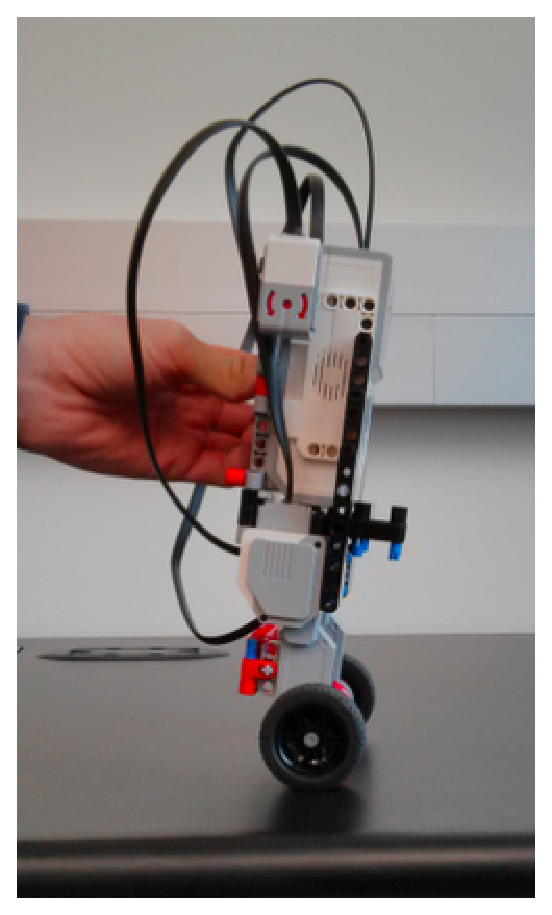
\includegraphics[width=1in]{pics/Lego/Build_side2.eps}}
      \mbox{\emph{(b)}}
    \end{minipage}
  \end{center}
  \caption{Inverted Pendulum System}
  \label{fig:system_simulation}
\end{figure}
\FloatBarrier

This document provides detailed design and implementation information.

\section{Specifications}
The goal of the system is to make the pendulum stay at upright position, not falling down, by move
the pendulum's base back and forth when necessary. The only meaningful number we can give out is the
desired angle for the pendulum, which is 0 degree. Due to the fact that we have linearized our model from a
nonlinear model, as we will show in the next section, system can only work for small angles. 
Which means when the pendulum lean too much,
our model will be extremely inaccurate. Thus we have to make sure our system output's rise time
to be as small as possible, oscillation is allowed as long as it eventually settles.

\section{Modeling}

The pendulum can rotate forward and backward freely. The base of pendulum is connected to two wheels
whose movements are identical which means the base of the pendulum is only capable moving in two
directions. We are able to control the wheels by giving it an angular acceleration forward or
backward. 

\begin{figure}[!h]
  \begin{center}
    \includegraphics[width=2 in]{pics/Full_System_2.eps}
  \end{center}
  \caption{System setup for inverted pendulum}
  \label{fig:full_system}
\end{figure}

\subsection{X-axis}
On the horizontal, x-axis, we have:

\begin{align*}
  % F_x & = F_{cart} + F_{rod} \\
  % F_{cart} & = M\ddot{x}  \\
  % F_{rod}  & = m a_x + m a_{p} \\
  %         & = m \ddot{x} + m (a_{t} + a_{c})
  F_x & = (M+m) \ddot{x} + m (a_{t} + a_{c})
\end{align*}

where $a_t$ and $a_c$ are tangential and centripetal acceleration respectively. 

\begin{figure}[!h]
  \begin{center}
    \begin{minipage}[b]{3.5in}
      \centerline{\mbox{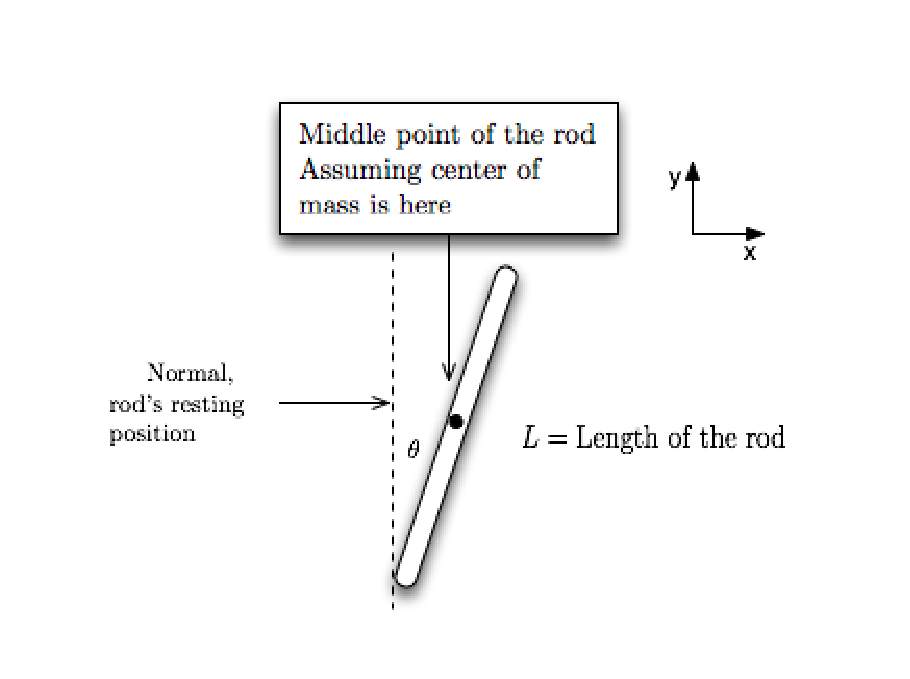
\includegraphics[width=3.5in]{pics/rod.eps}}}
    \end{minipage}
    \begin{minipage}[b]{3.5in}
      \centerline{\mbox{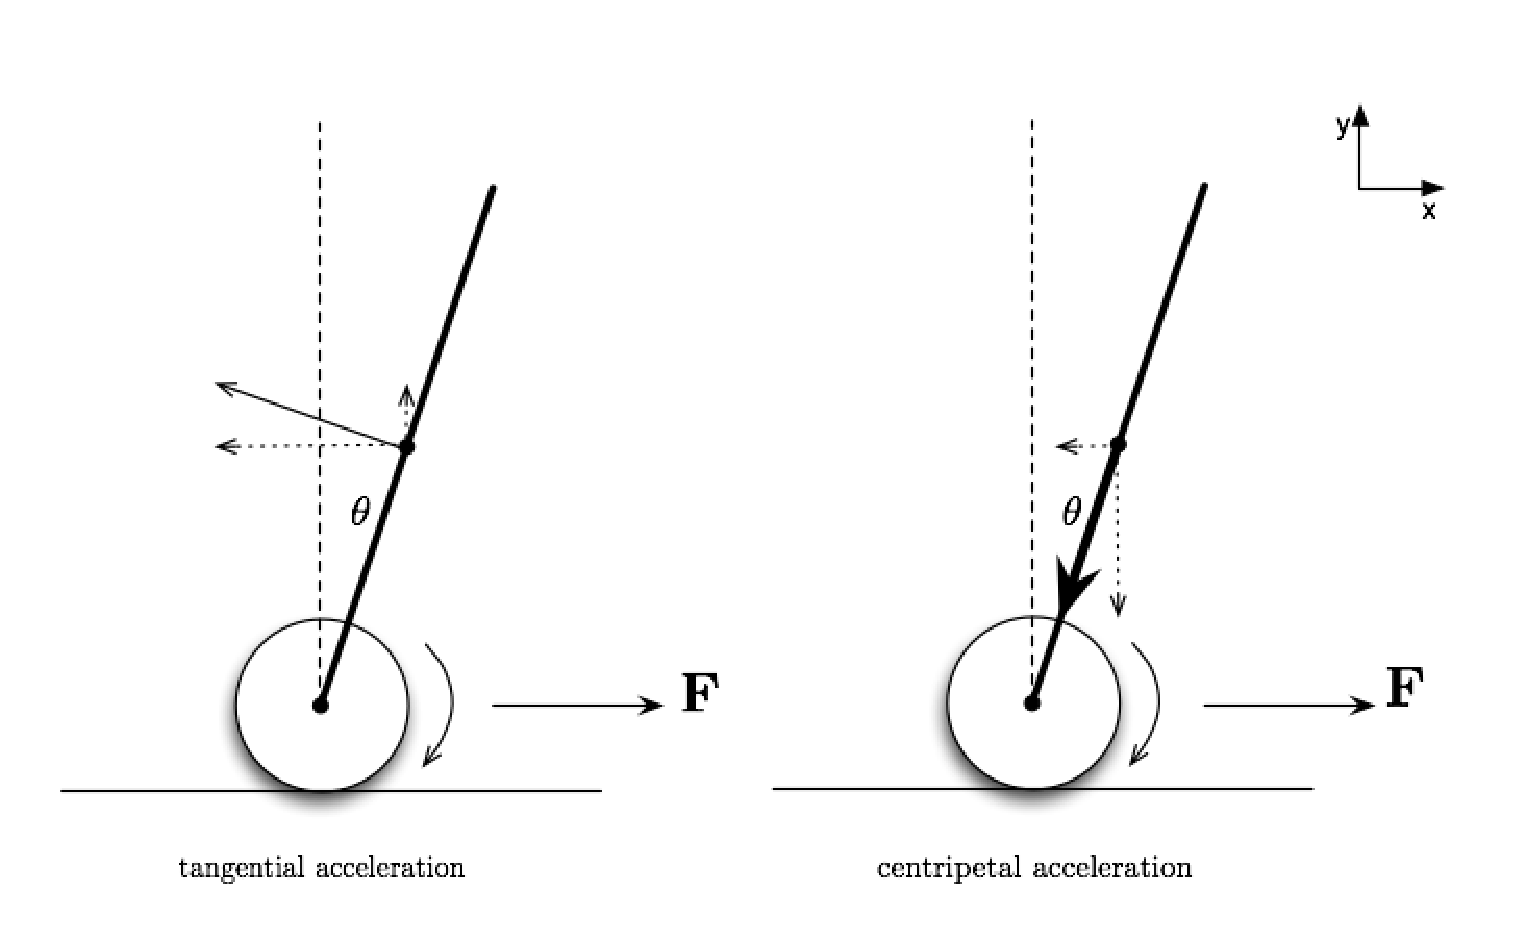
\includegraphics[width=4.5 in]{pics/rod_acc.eps}}}
    \end{minipage}
    
  \end{center}
  \caption{Angular acceleration disection for the rod}
  \label{fig:angular_rod}
\end{figure}

According to figure~\ref{fig:angular_rod}, angular accelerations for the rod on x-axis can be
expressed as:
\begin{align*}
  a_t & = -\dfrac{L}{2} \ddot{\theta} \\
  a_c & = -\dfrac{L}{2} \dot{\theta}^2
\end{align*}

Since we are only interested in the components on the x-axis, we have:

\begin{align*}
  a_t & = -\dfrac{L}{2} \ddot{\theta} \cos \theta \\
  a_c & = -\dfrac{L}{2} \dot{\theta}^2 \sin \theta
\end{align*}

So 

\begin{align}
  F_x & = (M+m) \ddot{x} + m (a_{t} + a_{c})\nonumber\\
         & = (M+m) \ddot{x} -m\dfrac{L}{2} \ddot{\theta} \cos \theta 
                        -m\dfrac{L}{2} \dot{\theta}^2 \sin \theta 
%	      & = (M + m) \ddot{x} - m\dfrac{L}{2} \ddot{\theta} \cos \theta 
%	                     - m \dfrac{L}{2} \dot{\theta}^2 \sin \theta
\end{align}
\FloatBarrier


\subsection{Y-axis}
Using Newton's second law for the vertical motion of the pendulum gives

\begin{align*}
  % F_y & = ma_y - mg \label{eqn:eq1} \\
  F_y & = ma_y - mg \\
      & = m(a_t + a_c) - mg
\end{align*}
where $a_y$, $a_t$ and $a_c$ are acceleration of y-axis, tangential and centripetal of the rotation
respectively. 

Using figure~\ref{fig:angular_rod}, we can express the acceleration on y-axis with:
\begin{align*}
  a_t & = \dfrac{L}{2}\ddot{\theta}\sin\theta \\
  a_c & = -\dfrac{L}{2}\dot{\theta}^2\cos\theta
\end{align*}

So

\begin{align}
  F_y & = m(a_t + a_c) - mg \nonumber\\
      & = m(\dfrac{L}{2}\ddot{\theta}\sin\theta - \dfrac{L}{2}\dot{\theta}^2\cos\theta) - mg
      \nonumber\\ 
      & = m\dfrac{L}{2}\ddot{\theta}\sin\theta - m\dfrac{L}{2}\dot{\theta}^2\cos\theta - mg
       \label{eqn:f_y}
\end{align}

 % Since $ y = \dfrac{L}{2}\cos\theta$,

 % \begin{align}
 %   \dot{y} & = \frac{d(l/2\cos\theta)}{dt} = -\dfrac{L}{2}\ddot{\theta}\sin\theta \nonumber\\
 %   % \frac{dy_G}{dt} & = \frac{d(l/2\cos\theta)}{dt} = -l/2\sin\theta\frac{d\theta}{dt} \nonumber\\
 %   \frac{d^2y_G}{dt^2} & = \frac{d}{dt}\left(-l/2/2 \sin\theta \frac{d\theta}{dt}\right) \nonumber\\
 %   & = -l/2/2\left(\frac{d\sin\theta}{dt}\frac{d\theta}{dt} + \sin\theta\frac{d^2\theta}{dt^2}\right) \nonumber\\
 %   & = -l/2\left( \cos\theta \left(\frac{d\theta}{dt}\right)^2 + \sin\theta\frac{d^2\theta}{dt^2}   \right) \nonumber\\
 %   & = -l/2\cos\theta\left(\frac{d\theta}{dt}\right)^2-l/2\sin\theta\frac{d^2\theta}{dt^2}\label{eqn:eq2}
 % \end{align}
 
 % Using Equation~\ref{eqn:eq2}, Equation~\ref{eqn:eq1} can be written as 
 % \begin{align*}
 %   F_y - mg & = m(-\frac{L}{2}\dot{\theta}^2\cos\theta - \frac{L}{2}\ddot{\theta}\sin\theta )
 % \end{align*}
 
 % Thus, the vertical reaction force, $F_y$, can be written as
 % \begin{align*}
 %   F_y & = mg + m\left(-\frac{L}{2}\dot{\theta}^2\cos\theta - \frac{L}{2}\ddot{\theta}\sin\theta\right)
 % \end{align*}

 \subsection{Angular Momentum}
 
 For any object, the relationship between the moment applied on an object and its angular acceleration is given by the following relationship
 \begin{align}
   I \ddot{\theta} = \sum \overline{M} \label{eqn:torque}
 \end{align}
 
 where $\overline{M}$ is the moment due to a given force and defined as 
 
 \[
 \overline{M} = \vec{F} \times \vec{r}
 \]
 
 where $\vec{F}$ is the force vector, $\vec{r}$ is the position vector of the object with respect to
 the point about which the moments are being summed, and $I$ is the angular momentum of the object.
 For the pendulum, summing the moment around the center of gravity, Equation~\ref{eqn:torque} can be
 written as

 \begin{eqnarray*}
   I\ddot{\theta} & = & F_y\dfrac{L}{2}\sin\theta - F_x\dfrac{L}{2}\cos\theta \\
     & = & \left( m\dfrac{L}{2}\ddot{\theta}\sin\theta - m\dfrac{L}{2}\dot{\theta}^2\cos\theta 
            - mg\right) \dfrac{L}{2}\sin\theta \\
     &   & -\left( (M+m)\ddot{x} - m\dfrac{L}{2}\ddot{\theta}\cos\theta - 
             m\dfrac{L}{2}\dot{\theta}^2\sin\theta \right) \dfrac{L}{2}\cos\theta\\
     & = & m\dfrac{L^2}{4}\ddot{\theta}\sin^2\theta 
           - \cancel{m\dfrac{L^2}{4}\dot{\theta}^2\cos\theta\sin\theta} - \dfrac{L}{2}mg\sin\theta\\
     &   & - (M+m) \dfrac{L}{2} \ddot{x}\cos\theta + m\dfrac{L^2}{4}\ddot{\theta}\cos^2\theta + 
             \cancel{m\dfrac{L^2}{4}\dot{\theta}^2\sin\theta\cos\theta} \\
     & = & m\dfrac{L^2}{4}\ddot{\theta}\cancelto{1}{(\sin^2\theta + \cos^2\theta)}
           - \dfrac{L}{2}mg\sin\theta - (M+m) \dfrac{L}{2}\ddot{x}\cos\theta \\
     & = & m \dfrac{L^2}{4}\ddot{\theta} - \dfrac{L}{2}mg\sin\theta 
           - (M+m) \dfrac{L}{2} \ddot{x}\cos\theta
    %               & = & (mg 
    %                    + m(-l\ddot{\theta}\cos\theta - l\ddot{\theta}\sin\theta)
    %                   )l\sin\theta 
    %                   -m(\ddot{x} 
    %                       - \ddot{\theta}l\sin\theta + \ddot{\theta}l\cos\theta
    %                   )l\cos\theta \\
    % & = & mgl\sin\theta - ml^2\ddot{\theta}\cos\theta\sin\theta- ml^2\ddot{\theta}\sin^2\theta \\
    % &  & - ml\ddot{x}\cos\theta + ml^2\ddot{\theta}\cos\theta\sin\theta 
    %     - ml^2\ddot{\theta}\cos^2\theta \\
    % & = & mgl\sin\theta - ml^2\ddot{\theta}(\sin^2\theta + \cos^2\theta) - ml\ddot{x}\cos\theta \\
    % & = & mgl\sin\theta - ml^2\ddot{\theta} - ml\ddot{x}\cos\theta 
 \end{eqnarray*}

We are assuming the center of gravity and the center of mass of the rod are at the same point, so
there is no angular movement of the rod around it's center. Therefore:

\begin{align}
  I\ddot{\theta} & = 0 \nonumber\\
  m \dfrac{L^2}{4}\ddot{\theta} - \dfrac{L}{2}mg\sin\theta 
      - (M+m) \dfrac{L}{2} \ddot{x}\cos\theta  & = 0 \nonumber\\
  m\dfrac{L}{2}\ddot{\theta} - mg\sin\theta - (M+m)\ddot{x}\cos\theta & = 0 \nonumber\\
  \eqnote{since} x = \omega r & \nonumber\\
  m\dfrac{L}{2}\ddot{\theta} - mg\sin\theta - (M+m)\dot{\omega}r\cos\theta & = 0 \nonumber
\end{align}

Using linear approximation, we approximate:

\begin{align}
  m\dfrac{L}{2}\ddot{\theta} - mg\theta - (M+m)\dot{\omega}r & = 0 \label{eqn:pre_tf} \\ 
  & \begin{cases}
    \sin\theta \approx \theta \nonumber\\
    \cos\theta \approx 1\nonumber\\
  \end{cases}
\end{align}
 
\noindent Taking Laplace transform of equation~\ref{eqn:pre_tf}, we have: 

\begin{align*}
  m\dfrac{L}{2}s^2\Theta - mg\Theta & = (M+m)\Omega \\
  \Theta & = \dfrac{(M+m)r}{m}\dfrac{\frac{2}{L}}{s^2 - \frac{2g}{L}}\Omega
\end{align*}
where $\Omega$ is an input acceleration (replacing $\dot{\omega}$)\\

\noindent We now have the following transfer function:

\[
  T(s) = \dfrac{\Theta}{\Omega} = \dfrac{(M+m)r}{m}\dfrac{\frac{2}{L}}{s^2-\frac{2g}{L}}
\]

\begin{figure}[!h]
  \begin{center}
    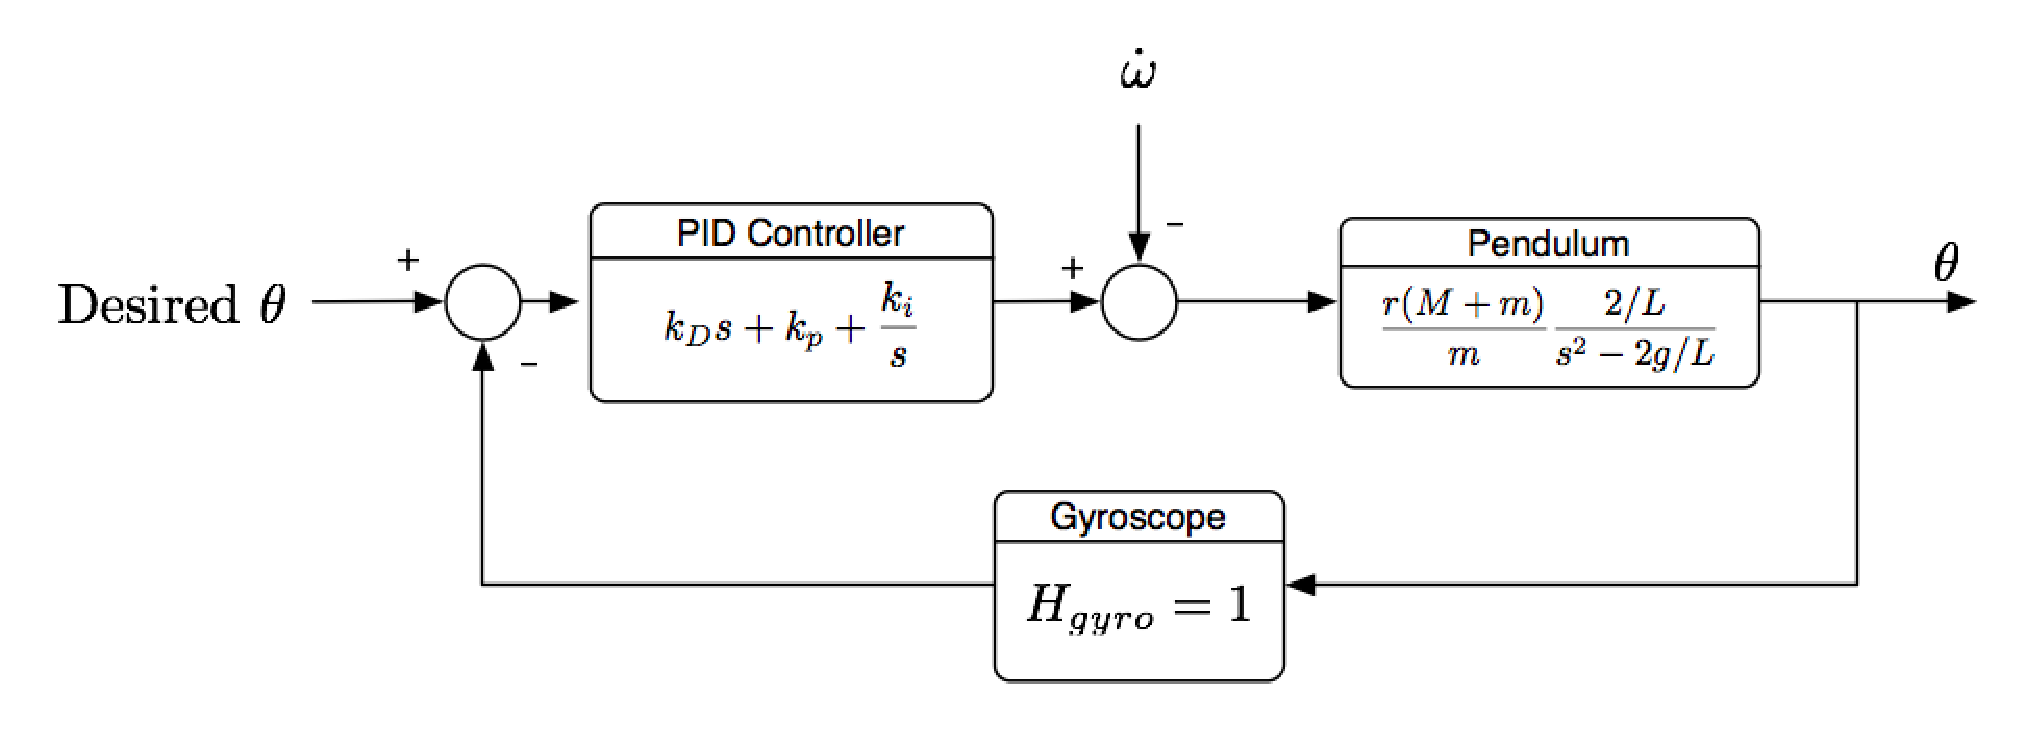
\includegraphics[width=5 in]{pics/Block_Diagram_2.eps}
  \end{center}
  \caption{Block diagram for our system}
  \label{fig:block_diagram}
\end{figure}

\begin{figure}[!h]
  \begin{center}
    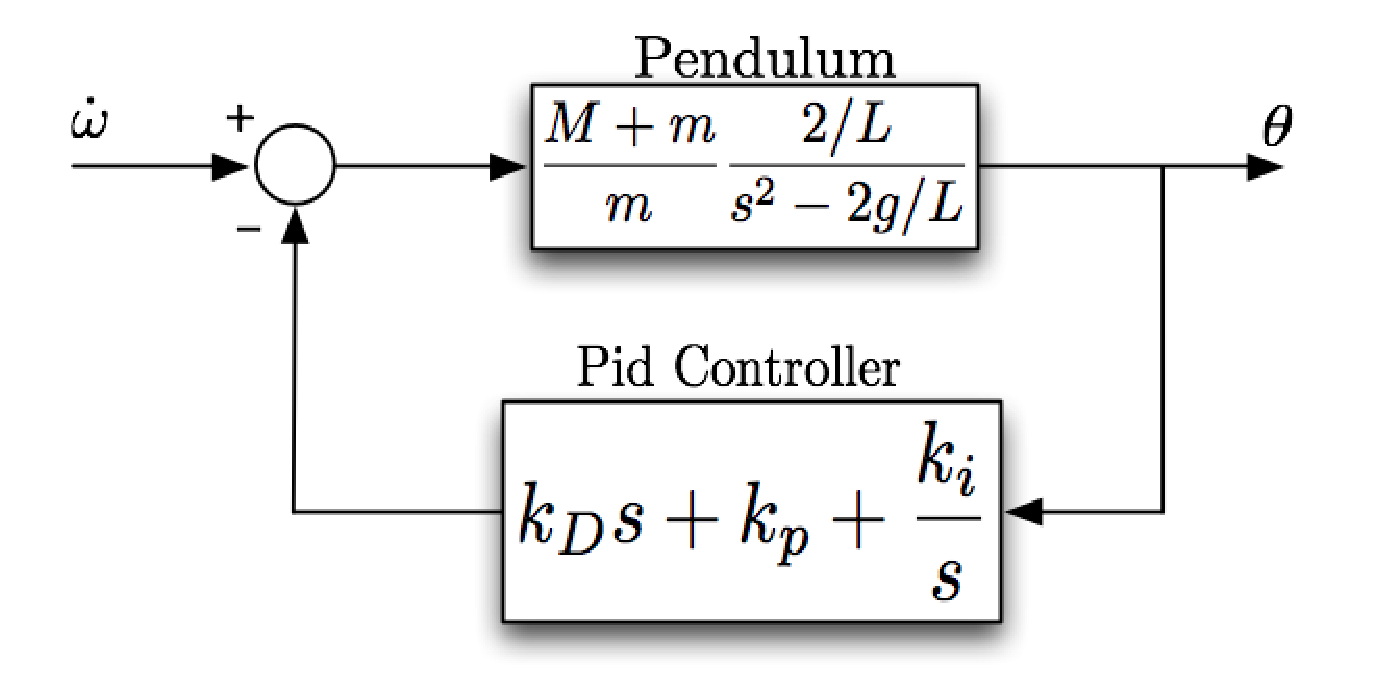
\includegraphics[width=4 in]{pics/Block_Diagram_3.eps}
  \end{center}
  \caption{Another way to understand  our system}
  \label{fig:block_diagram_3}
\end{figure}

We used Matlab to tune $K_p$, $K_D$, and $K_i$, giving them values of $K_D=20$, $K_p=300$, and $K_i=1$. We are estimating the friction coefficient to be about 0.8. This is tentative, however.

We can redraw this block diagram in the way shown on the next page. This is a different but equally valid  way of conceptualizing our system. In this system, the desired $\theta$ has been removed since it is equal to 0. The input to our system is now the disturbance acceleration, while  the PID controller is in the feedback loop. The gyroscope has been removed for additional simplification. 

\section{Performance Measurements}
The system was simulated in Matlab. The impulse response and bode plot are shown next. The design criteria require that the settling time be less than 5 seconds and that the pendulum should not move more than 0.05 radians away from the vertical axis. As seen in the impulse response, both design criteria have been met. The settling time was found to be 1.22 seconds.

\begin{figure}[!h]
  \begin{center}
    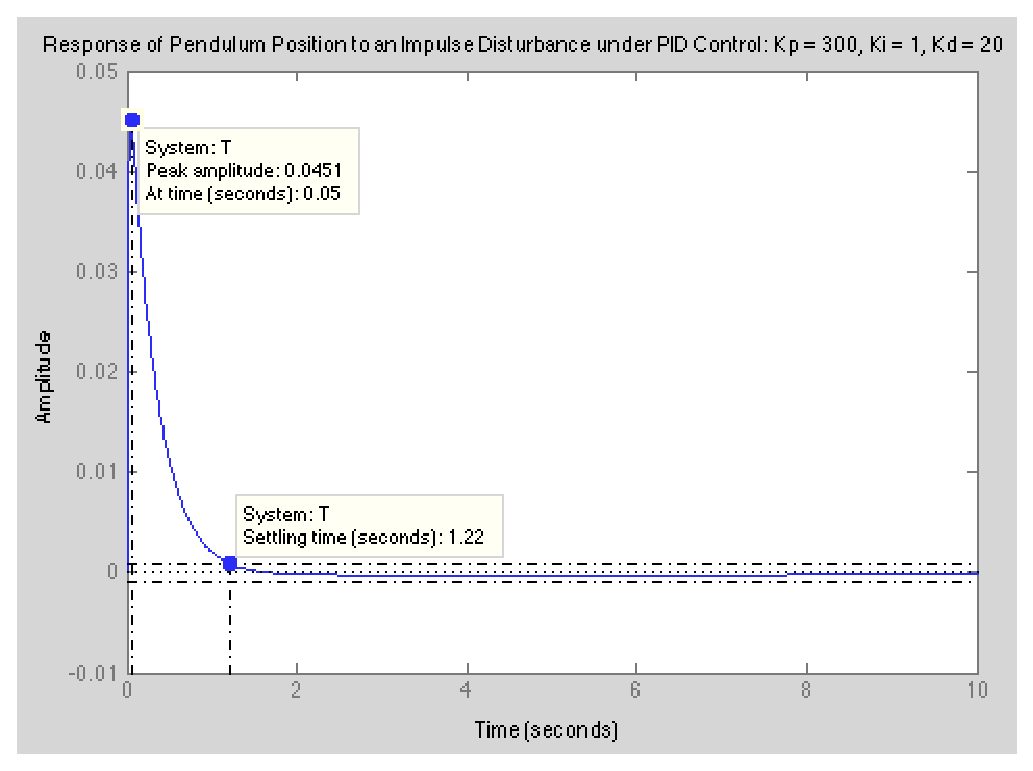
\includegraphics[width=4.5 in]{pics/performance_measurements/impulse_response_perf.eps}
  \end{center}
  \caption{Impulse response of our system}
  \label{fig:impulse_response}
\end{figure}

\begin{figure}[!h]
 \begin{center}
   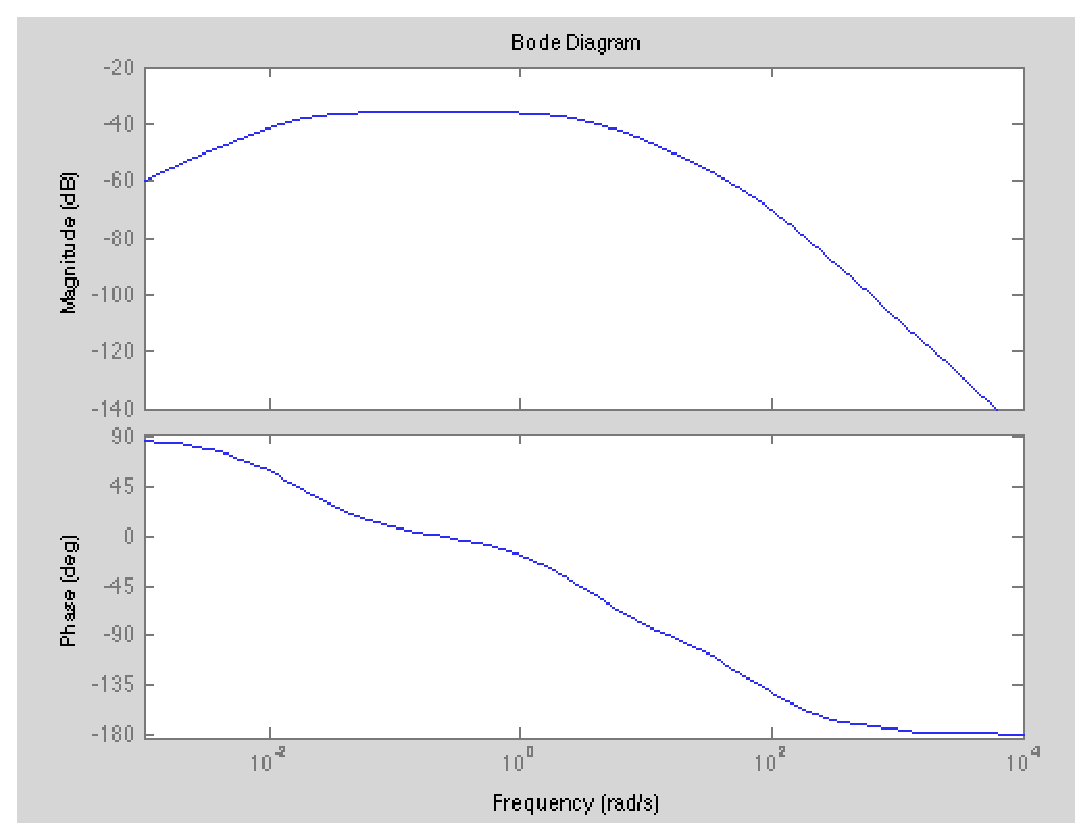
\includegraphics[width=4.5 in]{pics/performance_measurements/bode_plot.eps}
 \end{center}
 \caption{The Bode plot of our system.}
 \label{fig:bode_plot}
\end{figure}

\begin{figure}[!h]
  \begin{center}
    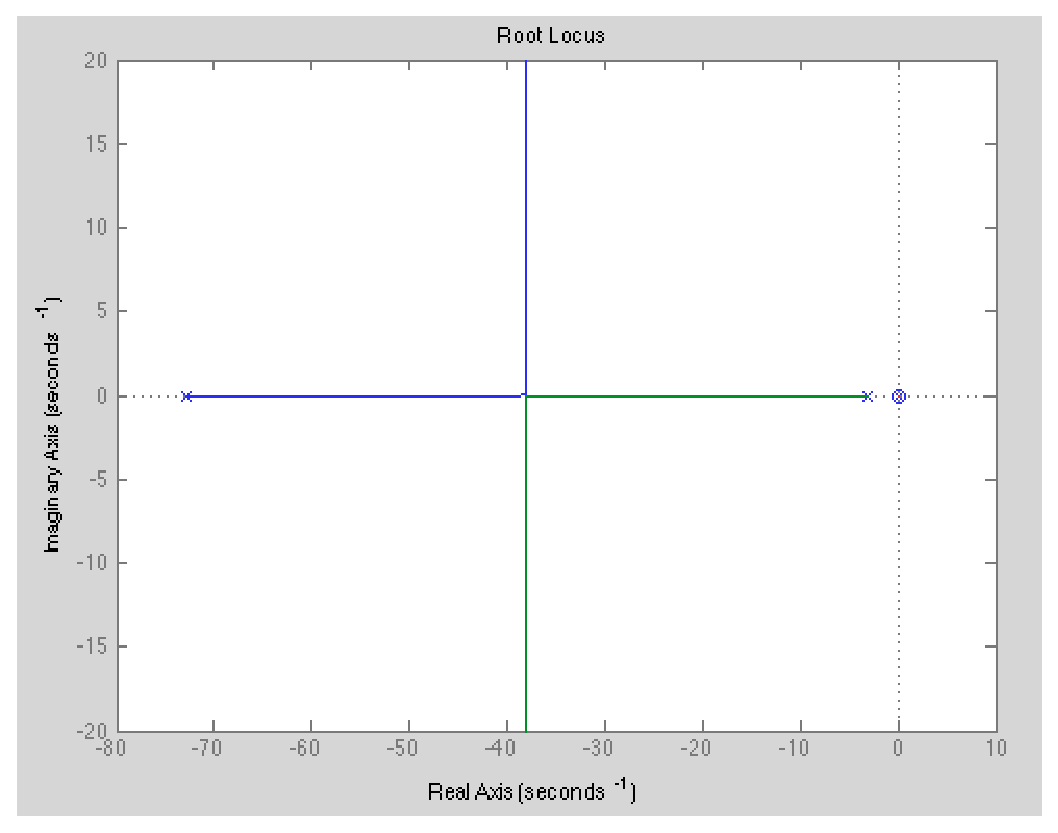
\includegraphics[width=4.5 in]{pics/performance_measurements/root_locus.eps}
  \end{center}
  \caption{The root locus plot}
  \label{fig:root_locus}
\end{figure}

Here is the Matlab code:
\SourceCode{Matlab}{Matlab code for tuning}{lst:tuning}{../Matlab/PID_Design.m}

\section{Implementation}

The system is implemented on a Lego Mindstorm EV3 running LeJOS 0.4 alpha as it's operating system. 
The OS comes with a embedded version of JVM. There is also a Java library interfacing with all
hardware components.

Since we are implementing a PID controller, the physical model does not matter at this point. 
We can treat the physics and the gyro sensor as a black box, when given a angular acceleration as
input an corresponding output is given by the gyro sensor's reading. What really masters is the PID
controller.

For our PID controller the derivative of error of desired angle can be obtained by an additional
gyro sensor. As it turns out each gyro sensor has two modes, one is angle mode, measuring the angle
from initial position, the other is the rate mode, measuring the rate of change of angles. The
integral is calculated by summing up all the errors. 

The challenge of the implementing PID controller is to choose a set of appropriate parameters. This
could be done in several ways. One is the well known Ziegler-Nichols method which is doing the
following steps: 
\begin{enumerate}
  \item Set all gains to zero.
  \item Increase the P gain until the response to a disturbance is steady oscillation. 
  \item Increase the D gain until the the oscillations go away (i.e. it's critically damped).
  \item Repeat steps 2 and 3 until increasing the D gain does not stop the oscillations.
  \item Set P and D to the last stable values.
  \item Increase the I gain until it brings you to the setpoint with the number of oscillations desired 
\end{enumerate}

This did not work well from start, as we could not find a value of P that make the system has steady
oscillation. So we try a different one:

\begin{enumerate}
\item Set all gains to 0.
\item Increase $K_d$ until the system oscillates.
\item Reduce Kd by a factor of 2-4.
\item Set $K_p$ to about $1\%$ of $K_d$.
\item Increase Kp until oscillations start.
\item Decrease Kp by a factor of 2-4.
\item Set $Ki$ to about $1\%$ of $K_p$.
\item Increase Ki until oscillations start.
\item Decrease Ki by a factor of 2-4.
\end{enumerate}

We were able to find a $K_d$ that make the system close to steady oscillation, as we had to give it a
little push. But after that, it's hard to find any satisfiable value. 


\section{Failure Analysis}

There are many reasons we could not find the parameters. Time constrain and lack of experience
probably do count for quite a bit, but I also think there could some design issues. The main
processor unit of the Lego is quite heavy, and it's placed quite high relative to the wheels. So the
center of gravity is very high. This make the system very sensitive, thus require fairly precise set
of parameters in order to be stable. Also, our input acceleration is in terms of wheels' rotation.
But what really counts is the acceleration on horizontal axis which depending on the radius of the
wheels. Thus, with a design having lower center of gravity and larger wheels can probably make the
parameters much easier to find.


\section*{Source Code}
% The effect of our modeled transfer function is now the real physics, giving an
% acceleration to the base of the pendulum, we should have an change of angle. So the real challenge
% here is to tune to PID controller to a state that come make the pendulum staying upright. 

% We have tried Ziegler–Nichols method, which start with tuning $Kp$, and a different method that
% start with tuning $Kd$. With the second method, the system have come to a state very close to
% oscillating around center position. But due to time constrain and lack of experience we were unable
% to find a suitable parameters.

\SourceCode{Java}{class for reading gyro sensor}{lst:gyro}{../src/Gyro.java}
\SourceCode{Java}{main pendulum class}{lst:gyro}{../src/Pendulum.java}

\end{document}
